\documentclass[12pt]{article}
\usepackage{xeCJK}

\usepackage{charter}
\usepackage{fullpage}
\usepackage[colorlinks=false]{hyperref}
\usepackage{ifthen}
\usepackage{comment}
\usepackage[title,titletoc]{appendix}
\usepackage{pagecolor}
\usepackage{amsmath}
\usepackage{amsfonts}
%\usepackage[normalem]{ulem}
%\usepackage{siunitx}
\usepackage{amsthm}

%\sisetup{per=slash, load=abbr}

\usepackage{paralist}
\usepackage{pgfplots}
\usetikzlibrary{positioning}
\usetikzlibrary{fit}
\usetikzlibrary{snakes}
\usetikzlibrary{shapes.geometric}
\usetikzlibrary{patterns}
\usetikzlibrary{shapes,arrows,chains}
\usepgfplotslibrary{patchplots,colormaps}
\usetikzlibrary{calc}
\usetikzlibrary{positioning, fit}
\usetikzlibrary{backgrounds}
\usetikzlibrary{intersections}

\newcommand{\whitepaper}[1]{\begin{center}\fbox{\parbox{0.75\textwidth}{{\small
#1}}}\end{center}}

\newcommand{\pcolor}{white!25}

\usepackage{setspace}
\usepackage[ruled,vlined]{algorithm2e}
\bibliographystyle{ieeetr}

\usepackage{geometry}
\geometry{left=3cm,right=3cm,top=1.6cm,bottom=3cm,headheight=20pt,headsep=1.5em}
\usepackage{fancyhdr}
\pagestyle{fancy}
\chead{
\includegraphics[scale=0.1]{../common/logo.png}  
\includegraphics[scale=0.1]{../common/yeez.png}}  %在此处插入logo.pdf图片 图片靠左
\lhead{} % 页眉中间位置内容
\rhead{}
\usepackage{expl3}
\ExplSyntaxOn
\newcommand\latinabbrev[1]{
  \peek_meaning:NTF . {% Same as \@ifnextchar
    #1\@}%
  { \peek_catcode:NTF a {% Check whether next char has same catcode as \'a, i.e., is a letter
      #1.\@ }%
    {#1.\@}}}
\ExplSyntaxOff

%Omit final dot from each def.
\def\eg{\latinabbrev{e.g}}
\def\etal{\latinabbrev{et al}}
\def\etc{\latinabbrev{etc}}
\def\ie{\latinabbrev{i.e}}
\newcommand{\dapp}{DApp\xspace}

%\setlength{\topskip}{1em}

\usepackage{indentfirst}
\usepackage{amssymb}
\usepackage{exscale}
\usepackage{relsize}
\usepackage{float}
%\usepackage[ruled,vlined]{algorithm2e}

\setCJKmainfont[BoldFont = STSongti-SC-Bold]{STSongti-SC-Regular}
\setCJKfamilyfont{hei}{SIL-Hei-Med-Jian}		%宋体
\setCJKfamilyfont{song}{SimSun}		%宋体
\setCJKfamilyfont{kai}{Kaiti}		%楷体
\setCJKfamilyfont{fang}{song}	%仿宋
\setCJKfamilyfont{li}{song}			%隶书
\setCJKfamilyfont{you}{Yuanti}		%幼圆

\newcommand{\song}{\CJKfamily{song}}	%宋体
\newcommand{\hei}{\CJKfamily{hei}}	%黑体
\newcommand{\kai}{\CJKfamily{kai}}	%楷体
\newcommand{\fs}{\CJKfamily{fang}}	%仿宋
\newcommand{\li}{\CJKfamily{li}}		%隶书
\newcommand{\you}{\CJKfamily{you}}	%幼圆
\newcommand{\reffig}[1]{图\ref{#1}}
\newcommand{\refsec}[1]{\S~\ref{#1}}

\newcommand{\txhash}[1]{{\href{https://etherscan.io/tx/#1}{\texttt{#1}}}}

\onehalfspacing   % ----------设置1.5倍行距(可能有意义,待调整)

%\parindent=20pt  % -------------------首行缩进大小,英文分段就直接0pt了吧。
\setlength{\parindent}{2.1em}
\setlength{\parskip}{0.3\baselineskip}
\newcommand{\nrcore}{Core Nebulas Rank}
\newcommand{\nrext}{Extended Nebulas Ranks}
\newcommand{\dom}{{\; \texttt{dom}\;}}
\newcommand{\nr}{\Gamma}
\newcommand{\ec}{椭圆曲线}
\newcommand{\ds}{\{0,...,d\}}
%\newcommand{\pp}{$\mathcal{P}$}
%\newcommand{\vv}{$\mathcal{V}$}
\newcommand{\oo}{\mathcal{O}}
\newcommand{\fp}{\mathbb{F}_p}
\newcommand{\fpn}{\mathbb{F}_{p^n}}
\newcommand{\fpk}{\mathbb{F}_{p^k}}
\newcommand{\fq}{\mathbb{F}_q}
\newcommand{\ebk}{E(\bar{\mathbb{K}})}
\newcommand{\bfp}{\bar{\mathbb{F}}_p}

\setCJKsansfont[BoldFont = STHeitiSC-Medium]{STHeitiSC-Light}


\newtheorem{property}{特征}
\newtheorem{corollary}{推论}
\newtheorem{assumption}{假设}
\newtheorem{definition}{定义}
\newtheorem{remark}{注}[section]
%\addbibresource{reference.bib}

\begin{document}
\pagestyle{empty}
\renewcommand{\contentsname}{目录}
\renewcommand{\abstractname}{摘要}
\renewcommand{\refname}{参考文献}
%\renewcommand{\nomname}{术语表(按首字母排序)}
\renewcommand{\figurename}{图}
\renewcommand{\tablename}{表}
\renewcommand{\baselinestretch}{1.5}
\renewcommand{\appendixname}{附录}
\renewcommand{\proofname}{证明}

\pagecolor{\pcolor}



\begin{titlepage}
  \begin{center}
    \vspace*{2.5cm}
    
\includegraphics[scale=0.2]{../common/logo.png}\\
    
\includegraphics[scale=0.2]{../common/yeez.png}

    \vspace{3.5cm}




   \textbf{\huge{椭圆曲线科普}}

    \vspace{2.5cm}
    ASResearch\\
    YeeZTech
    \textbf{}
  \end{center}

\end{titlepage}
\setcounter{page}{0}
%\thispagestyle{empty}
\tableofcontents
\newpage
\setcounter{page}{1}
\pagestyle{fancy}
\vspace*{0.01cm}

\section{总览}
说到椭圆曲线(EC,eclipse curve),任何一个区块链工作者可能并不陌生:他们可能知道BTC用椭圆曲线用于生成公私钥,管理签名等等,是保证BTC安全性的基础。更有甚者,他们可能知道椭圆曲线的基本群运算法则,是由两个点作直线与曲线相交在第三个点,然后再取x轴镜像来得到。事实上,因为市面上已经有相当完整的椭圆曲线计算工具,了解上述基本概念然后使用开源的库已经足以实现工程上的大量需求。

本文写作的初衷在于,通过调研椭圆曲线我们发现,之前接触到的仅仅只是冰山一角,其背后涉及的技术之广以及精妙程度远非我们所能想象。鉴于市面上大多介绍椭圆曲线技术的文章都是浅尝辄止,本文旨在做一种新的尝试:以最为通俗易懂的语言来介绍椭圆曲线关键定理以及精妙之处,让对数学/密码学感兴趣的读者开阔视野,一定程度上打破椭圆曲线技术的黑箱状态。

从实际角度来看,本文着重解释下面几个问题:
\begin{itemize}
	\item 为什么椭圆曲线会作为加密(包括签名)体系的首选。(相比于RSA,传统离散对数)
	\item 椭圆曲线计算的基本实现以及时间复杂度。
	\item pairing函数基本实现以及时间复杂度。(pairing作为zkSNARK的核心之一,是整个本文涉及技术,甚至是整个椭圆曲线技术的最高点之一,其定义会在之后介绍。)
\end{itemize}
值得一提的是,有人可能会说作为椭圆曲线工程上的实现并不需要理解上述问题,这的确是事实。但是即使是用别人的库,了解上述问题也确有可取之处:一方面有助于通读代码,另一方面可以掌握其背后的时间开销,对于做技术选型提供参考。同时,在理论层面,理解底层原理自然有助于吸收不断更新的区块链新技术。

本文的写作风格如下:鉴于其内容均为数学知识,本文以数学描述为主,但涉及的所有证明都会跳过,同时在描述基本定义与定理时使用“加工后的科普语言”,故存在大量不严谨不精确之处。我们会在下章介绍参考资料以便读者参阅严谨的表述。
\section{参考资料}
\begin{itemize}
\item "Elliptic Curves Number Theory and Cryptography“, Kenneth H.Rosen. 椭圆曲线技术的完整版教材,包含严谨的定义以及绝大部分证明。本文下一章的很多内容属于此书的解读。
\item "Pairing for beginners", Craig Costello. 专注于介绍pairing的科普教材。为了清晰表述此书已经处理成简单易懂的语言,且只包含少量证明,但长度仍有100多页。
\end{itemize}
\section{椭圆曲线基本概念}
\subsection{基本场景}
假设现在有一堆球摞在一起,其中最下面一层有$x^2$个球,倒数第二层$(x-1)^2$,以此类推。
\begin{figure}[H]
	\centering
	\label{fig:balls}
	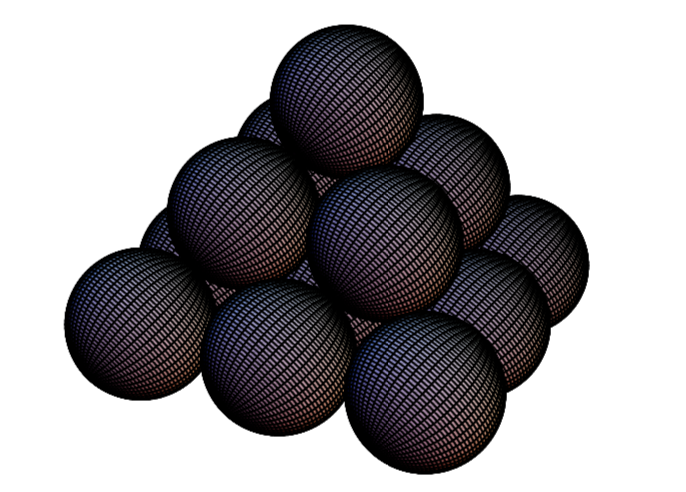
\includegraphics[width=0.4\textwidth]{../common/ball.png}
	%\includegraphics[width=0.6\textwidth]{2.png}
	\caption{球组成的金字塔}
\end{figure}
那么这些球的总数量为
$$1^2+2^2+3^2+...+x^2=\frac{x(x+1)(2x+1)}{6}$$
现在假设这个金字塔塌了,所有的球全部散落到一层。现在我们想知道这些散落的球能否组成一个正方形,即,是否存在一个整数$y$使得
$$y^2=\frac{x(x+1)(2x+1)}{6}$$
研究这样一个简单的问题虽然看似没有任何实际作用,但是它本质就是一个椭圆曲线的问题:方程的一边是关于$y$的二次多项式,另外一边是关于$x$的三次多项式,符合\ec 的基本形式。

科学家们在探索时发现,越来越多的实际问题均能转化成\ec ,例如

是否存在一个边长均为有理数的三角形面积为5。

这个问题可以通过换元转化成寻找下面这个方程的有理数解的问题,
$$y^2=x^3-25x$$
其也是一个椭圆曲线。

类似的,还有著名的费马大定理(6大数学难题之一),即当$n\geq 3$时,方程
$$a^n+b^n = c^n$$
没有除$(0,0,0)$之外的整数解。

该问题也可以通过换元转化为\ec 的问题。参考文献[1]介绍了该定理证明思路。
\subsection{基本形式}
根据上一章的表述,一个椭圆曲线要求$y$的次数不超过2,$x$的次数不超过3,其各项组合不外乎下面的形式
$$ y^2+a_1xy+a_3y=x^3+a_2x^2+a_4x+a_6$$
其中$a_1,...,a_6$为系数,其取值来源于一个固定的范围$\mathbb{K}$,可以理解成定义域。在绝大部分情形下,我们能够通过换元\footnote{当$\mathbb{K}$这个域的特征值不等于2或3时可以进行转化。一个域$\mathbb{K}$的特征值定义为多少个乘法单位元(1)加起来等于加法单位元(0)。因为换元过程会引入类似$a/2,a/3$的变量,如果$\mathbb{K}$特征值为2或3,因为“$2=0$”,上述定义不合法,所以此时仍然需要用称为generalized Weierstrass equation来表示。这种情形在实际研究中少见。}将上述\ec 表达式 (称为generalized Weierstrass equation)转化成
$$y^2=x^3+Ax+B$$
的形式,称作Weierstrass equation。这也是本文专注研究的椭圆曲线基本形式。
\subsection{\ec 群运算}
我们用$E:y^2=x^3+Ax+B$来表示一个椭圆曲线,满足$E$方程的点$P=(x,y)$表示椭圆曲线上的点。一般而言在直角坐标系中$E$长下面这样
\begin{figure}[H]
	\centering
	\label{fig:ecshape}
	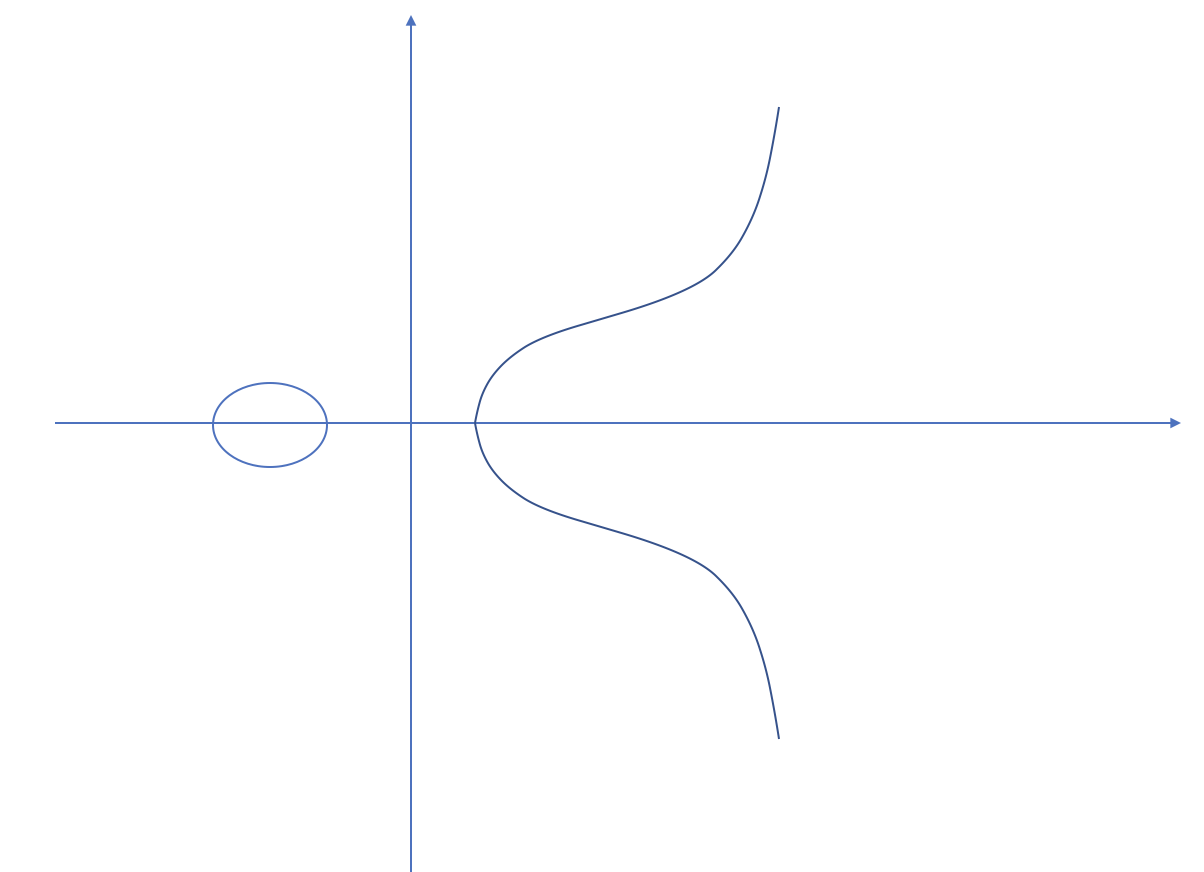
\includegraphics[width=0.6\textwidth]{../common/ecshape.png}
	%\includegraphics[width=0.6\textwidth]{2.png}
	\caption{\ec}
\end{figure}
我们发现这个曲线和$x$轴有三个交点,对应于方程$x^3+Ax+B=0$存在三个不同的根的情形。当然也有可能只有一个交点,对应方程$x^3+Ax+B$存在一个实根,两个虚根的情形。此时图\ref{fig:ecshape}左边的圆圈消失。如果$x^3+Ax+B=0$存在重根呢?我们不允许这种情况发生,即约定方程的判别式$4A^3+27B^2 \neq 0$。\footnote{三次方程的判别式$\delta=(r_1-r_2)(r_2-r_3)(r_3-r_1)$,其中$r_i$为方程的三个根。当且仅当判别式不为0时不存在重根。}

乍看之下,这个方程并没有什么特别之处,但是一旦将E上的点和群理论结合起来,我们会发现很多意想不到的巧妙性质,而这些性质也构成了\ec 的研究基础。

我们先回顾一下群的定义,大部分读者可能并不陌生:简单而言,群定义了一个集合和一个群运算,满足封闭性,结合律,存在单位元和逆元。

现在,我们把$E$ 上的所有点当做群的元素。当然,这些点的取值范围不一定是整个实数集(或复数),我们可以根据实际场景限制这些点的坐标(即方程的解)来源于一个域$L$,记作$E(L)$,表示这些点既要满足曲线的方程,同时取值也要属于域$L$。

然后,我们按照如下规则定义群的其他要素:
\begin{itemize}
	\item 我们定义一个无穷远点$\mathcal{O}$表示群的单位元。
	\item 我们注意到,经过$E$上任意两点的$P,Q$直线的必与$E$相交于第三点$R$。我们用加号$+$来表示群运算,然后让$P+Q$等于$R$关于$x$轴的对称点,作为群运算的结果。\footnote{如果$P=Q$,这条直线为点$P$对$E$的切线。当且仅当这条直线垂直于$x$轴时,定义第三个交点为无穷远点$\oo$,其关于$x$轴的对称点为它本身,即此时满足$P+Q=\oo$。}
	\item 对于$E$上的点$P$,其逆元素为$P$关于$x$轴的对称点,记作$-P$,亦即$P+(-P)=\mathcal{O}$
\end{itemize}
\begin{figure}[H]
	\centering
	\label{fig:grouplaw}
	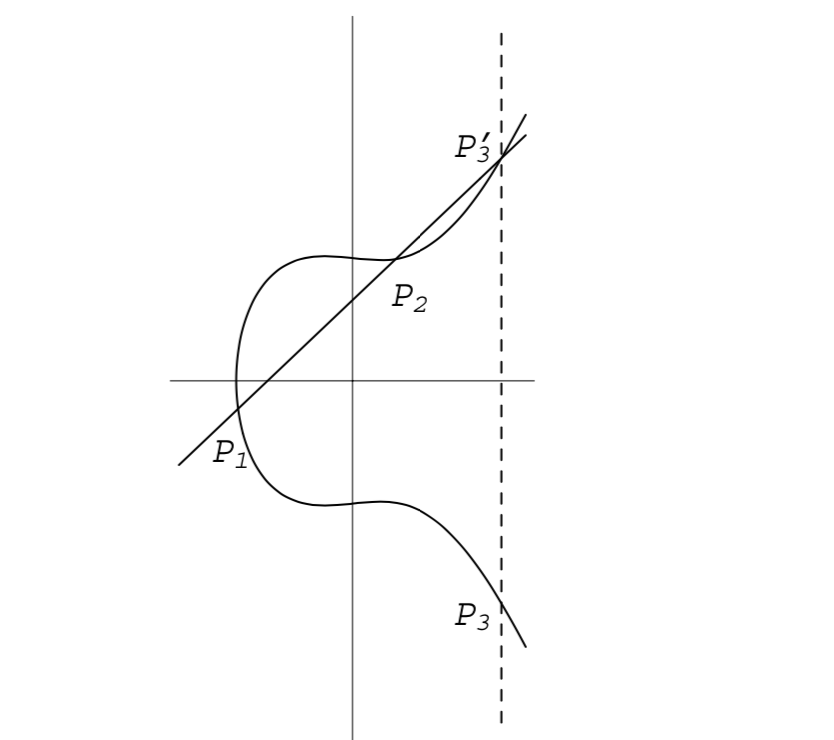
\includegraphics[width=0.6\textwidth]{../common/grouplaw.png}
	%\includegraphics[width=0.6\textwidth]{2.png}
	\caption{群运算}
\end{figure}
这样我们就给出了这个群的完整定义。在说明这个群确实满足群的各项要素之前,我们先通过下面的例子来说明如何求$P+Q$的具体坐标。

假设$P=(x_1,y_1),Q=(x_2,y_2)$,且$PQ$不垂直于$x$轴。则直线$PQ$的斜率$m=\frac{x_2-x_1}{y_2-y_1}$,方程为$y=m(x-x_1)+y_1$,带入$E$可得
$$(m(x-x_1)+y_1)^2=x^3+Ax+B,$$
展开得
$$x^3-m^2x^2+(\cdots)x+\cdots=0$$
上式是一个关于$x$的三次方程,且已知$x_1,x_2$为这个方程的两个解(因为$P,Q$既满足$E$的方程又满足直线方程。)。根据韦达定理可知,方程的三个解加起来一定等于二次项系数的相反数, \footnote{实际对于方程$ax^3+bx^2+cx+d=0$,三个根之和等于$-\frac{b}{a}$。在$a=1$时即为$-b$},故对于$R=(x_R,y_R)$,必有
$$x_R=m^2-x_1-x_2,$$
然后代入直线方程可求得
$$y_R=m(x_3-x_1)+y_1$$
根据定义,点$P+Q=(x_3,y_3)$为点$R$取关于$x$轴对称点。这只需将点$R$的$y$坐标取相反数即可,故我们得到
\begin{align}
\label{groupop}
& x_3 = m^2-x_1-x_2, y_3 = m(x_1-x_3)-y_1
\end{align}
上述情况对于$PQ$为切线时也成立,此时$x_1=x_2$,$m=\frac{3x_1^2+A}{2y_1}$。

当$PQ$垂直,即$x_1=x_2$时,定义$P+Q=\oo$,同时,当$P$或$Q$等于$\oo$时,根据单位元性质定义$P+\oo=P$。

根据(\ref{groupop})中描述的方式我们可以求出群运算的结果,而且我们不难发现,如果$P,Q\in E(L)$(recall:坐标的取值范围是域$L$),只要系数$A,B$也属于$L$,那么$P+Q \in E(L)$,满足了群的封闭性。

同时,不难发现这个群也满足交换性$P+Q=Q+P$\footnote{交换性不是构成群的必要条件。满足交换性的群叫做阿贝尔群}。

至此,我们只剩下结合律没有说明\footnote{群的结合律:$P+Q+R=P+(Q+R)$},而这也是整个群系统最为精妙的部分:有读者可能不能理解为什么不直接取第三个点的坐标(不做$x$轴镜像)作为群运算结果。事实上这样的定义无法满足结合律。而一些naive的满足结合律运算方式,如$(x_1,y_1)+(x_2,y_2) = (x_1+x_2,y_1+y_2)$或$(x_1x_2,y_1y_2)$(括号外面的$+$指定义的群运算,括号里面的$+$指两个数相加)等等,不能保证新计算出来的点也在$E$上。所以上述运算定义方式是完美契合椭圆曲线性质和群性质的方式!

结合律对于实际应用有什么作用呢?我们需要计算一个点的倍数时(若干次对自身的群运算),例如,计算
$$16P=\underbrace{P+P+...+P}_{16\mbox{个}}$$
时,我们可以依次算
$$2P=P+P,4P=2P+2P,8P=4P+4P,16P=8P+8P,$$
这就是所谓二分求幂的算法,只有满足结合律时才能使用。对于更一般的情况,可以通过下面的过程计算$kP$($k \in Z$),
\begin{enumerate}
	\item 初始化$a\leftarrow k, B \leftarrow \oo, C \leftarrow P$
	\item 如果$a$为偶数,$a \leftarrow a/2, B \leftarrow B, C \leftarrow 2C$
	\item 如果$a$为奇数,$a \leftarrow a-1, B \leftarrow B+C, C \leftarrow C$
	\item 如果$a \neq 0$,跳转到第二步。
	\item 输出$B$
\end{enumerate}
该方法能够让我们用$\log$级别的时间复杂度进行点倍数运算,是\ec 用于密码学技术的基础。

关于椭圆曲线结合律的证明在参考资料[1]中有介绍,其过程远比传统的加法,乘法运算的结合律要复杂,这里我们自然跳过。有兴趣的读者可以做下面的尝试:用Windows画图或者其他软件画一个椭圆,然后画一个内接六边形,然后将六边形的三组对边相交得到三个点,这三个点一定是\textbf{共线}的。
\begin{figure}[H]
	\centering
	\label{fig:pascal}
	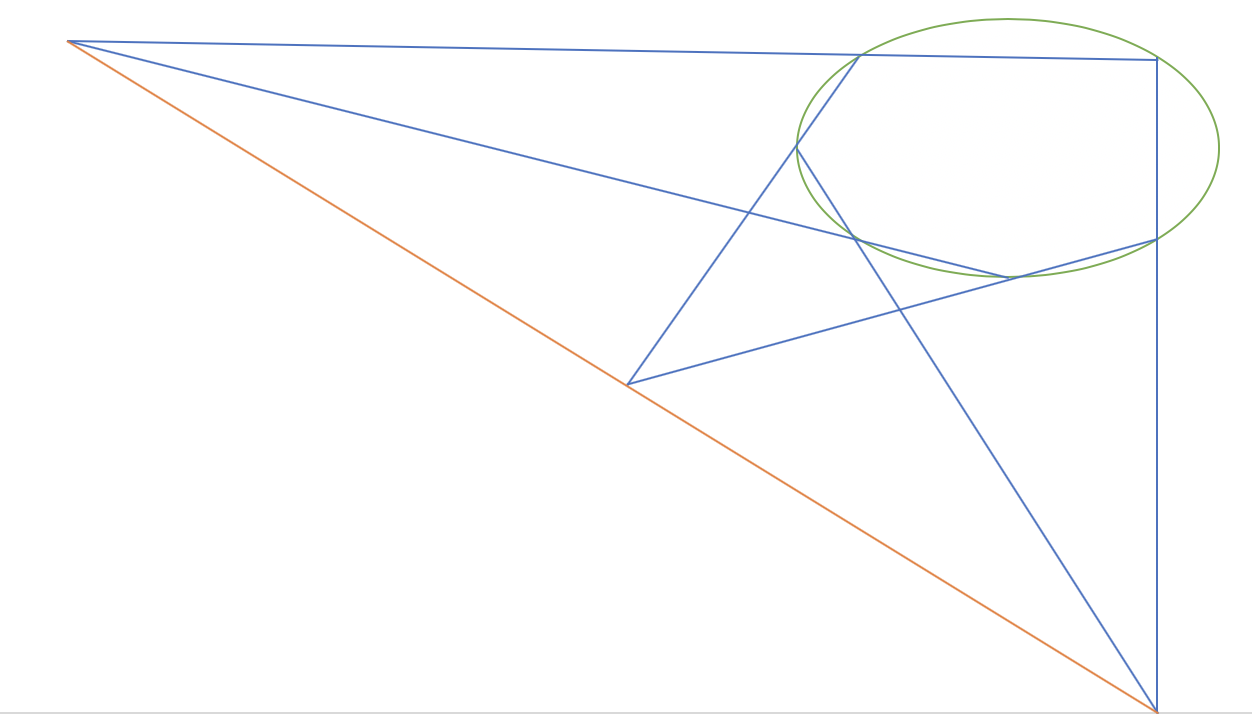
\includegraphics[width=0.7\textwidth]{../common/pascal.png}
	%\includegraphics[width=0.6\textwidth]{2.png}
	\caption{帕斯卡定理}
\end{figure}
学习过平面几何的读者可能知道这是所谓的帕斯卡定理。不过证明这个定理并不能证明椭圆曲线结合律。事实上帕斯卡定理以及怕普斯定理\footnote{帕斯卡定理中的椭圆退化成两条直线的情形}均是椭圆曲线结合律的推论。

有了完善的群系统和计算方法(\ref{groupop}),我们已经可以对\ec 的点进行任意操作。我们将在下章介绍\ec 的实际工程实现,其中用到了一些加速方法。这有助于我们读懂\ec 的开源代码,如\\“https://github.com/HarryR/solcrypto/blob/master/contracts/SECP2561k.sol”
\subsection{映射空间(Projective Space)}
一般而言一个二元组$(x,y)$即可表示一个\ec 上的点。现在我们做一个映射,对每个\ec 上的点,我们将它映射成一个三元组
$$(x,y) \rightarrow (x,y,1), ~\oo \rightarrow (0,1,0)$$
同时,对个三元组$(x,y,z)$,其中$x,y,z$不全为0,我们可以按照下面规则还原成二元组:
\begin{itemize}
	\item 如果$z \neq 0 $, $(x,y,z) \rightarrow (x/z,y/z)$
	\item 如果$z = 0$, $(x,y,0) \rightarrow \oo$
\end{itemize}
在此映射下\footnote{这个映射本质上是将二维坐标系中的点加上无穷远点映射到三维坐标系的直线。},我们把二元组上的运算转化为三元组上的运算,同时注意对于任意$\lambda \neq 0$,$(\lambda x, \lambda y, \lambda z)$表示的是同一个点。

使用三元组进行\ec 群运算的好处在于可以避免(\ref{groupop})中的除法计算——通常进行除法的时间复杂度是进行乘法的9至40倍。

当我们用三元组$P=(x_1,y_1,z_1),Q=(x_2,y_2,z_2)$来计算$P+Q=(x_3,y_3,z_3)$时,其计算方法如下:
\begin{itemize}
	\label{projectop}
	\item 如果$P \neq \pm Q$,那么
	$$	u = y_2z_1 −y_1z_2, v = x_2z_1 −x_1z_2, w = u^2z_1z_2 −v^3 −2v^2x_1z_2,$$
	$$x_3 = vw, y_3 = u(v^2x_1z_2 − w) − v^3y_1z_2, z_3 = v^3z_1z_2.$$
	\item 如果$P = Q$,那么
	$$ t=Az_1^2+3x_1^2, u=y_1z_1, v=ux_1y_1, w=t_2−8v,$$
	$$x_3 =2uw, y_3 =t(4v−w)−8y_1^2u^2, z_3 =8u^3.$$
	\item 如果$P = -Q$,那么$P+Q = \oo$
\end{itemize}
可以看到(\ref{projectop})的计算过程不包含任何除法,且不需要额外判断$P,Q$是否等于$\oo$,大大提高了计算效率。值得一提的是,\ec 点的三元组表示相比于二元组包含了额外的信息,故三元组表示只应出现在计算过程中。在储存和交互\ec 点的仍应使用二元组表示。
\subsection{\ec 于密码学中的应用}
上一章虽然介绍了椭圆曲线的群运算计算方法,然而如果我们不对$E$上的点做任何限制的话,随着计算的深入其坐标的数字化表示增长非常迅速,导致实际工程中难以进行记录。

在最基本的\ec 密码学工具里面,一般将系数$A,B$的取值以及\ec 点坐标的取值均限定在一个有限域$\mathbb{F}_p$中。这里$p$是一个很大的质数,通常有256位。而$\mathbb{F}_p=\{0,1,...,p-1\}$。这保证了\ec 点的取值来源于一个很大的范围,但是在实际工程中又是可表示,可计算的。

限定了定义域之后,上一章提到的所有四则运算操作均在模$p$意义下进行。在表达上不需要做任何修正。

有读者可能会问,反过来,是否所有满足方程$E$且$x,y \in \mathbb{F}_p$对应的椭圆曲线的点都包含在(上一章定义的)同一个\ec 群之内呢?这个答案是肯定的,可以有群运算的封闭性得到。这个群表示为$E(\fp)$。

\ec 加密体系的基础源于下面这个问题,即所谓的\ec 离散对数问题:

\textbf{给定$P,Q \in E(\mathbb{F}_p)$,找到$k \in \mathbf{Z}$使得$kP=Q$是困难的。\footnote{只能说对绝大部分\ec 而言。某些特殊的椭圆曲线存在计算离散对数的快速算法,具体见下一章。}}

这里$k$就是所谓的离散对数,而这里的困难是指目前还不存在低于指数级别的算法。注意之前提到通过$k,P$算$Q$可以通过二分求幂来算,是简单的。\ec 离散对数告诉我们这个过程不可逆。

目前破解\ec 离散对数问题最好的算法是$\sqrt{p}$级别,对于同样规模的加密体系,相比于传统离散对数\ec 拥有更高的安全性。具体原因我们会在下一大章介绍。

基于\ec 离散对数问题,通常,用户随机生成一个整数$s$作为私钥\footnote{这个$k$的取值范围应是不超过$E(\fp)$的阶,即过$E(\fp)$一共包含的\ec 点的个数。这个阶和$p$大小差不多,故仍是一个很大的数。其具体定义我们会在下一章介绍。}。然后,对于一个公共的生成元$P$\footnote{$P$是群$E(\fp)$的生成元,即从$P$出发每次加上自身,集合$\{P,2P,3P...\}$能够包含群$E(\fp)$所有元素(实际上等于$E(\fp)$)。},用户将$sP$作为公钥并公开。由于破解\ec 离散对数是困难的,对手(adversary)无法通过公钥计算出私钥的值。

值得一提的是,之后涉及$E(\fp)$中元素的系数的运算,均应在模$q$意义下进行,其中$q$为群$E(\fp)$的阶。如$abP = (ab \bmod q)P$。计算椭圆曲线点的坐标时仍在模$p$意义下进行。通常,可以认为$q$也是一个很大的质数且与$p$差不多大。椭圆曲线的系统提供方通常会附带给出参数$p,q,P$等。

我们接下来介绍基于\ec 的非对称(公私钥)加密体系。在那之前,我们需要介绍如何将一个信息$m$,通常可以用一个二进制数表示且不超过256位,编码成椭圆曲线上的点$(x,y)$。

注意到,直接将$m$映射成$x$可能行不通:$m^3+Am+B$可能在$\fp$下不是模$p$意义下的完全平方数,即不存在横坐标为$m$的$E(\fp)$元素。这里我们介绍比较通用的Koblitz编码方式。

\textbf{
给定待编码信息$m$,分别对$j=0,1,...,99, x_j = 100m+j, s_j = x_j^3+Ax_j+B$进行尝试直到满足$s^j$是模$p$意义下的完全平方数\footnote{判断方法为计算$s_j^{(p-1)/2}$看是否$\equiv 1 \bmod p$。这个成功概率是1/2。一旦验证通过,则当$p \bmod 4 =1 $时可通过$s_j^{(p-1)/4}$计算$y$;当$p \bmod 4 = 3$时,$y$也可计算但相对复杂,参考\\A course in computational algebraic number theory, volume 138 of Graduate Texts in Mathematics. Springer-Verlag, Berlin, 1993.},此时把$x_j$以及对应的$\sqrt{s_i}$分别作为\ec 上的点$(x,y)$。
同时,给定椭圆曲线上的点$(x,y)$,我们只需计算$m=[x_j/100]$(整除运算)来还原原始信息$m$。这个过程编码和解码的时间复杂度都是$O(1)$的且唯一确定。}

基于至此介绍的工具,我们接下来介绍常见的基于\ec 的加密和签名体系。以下我们约定$s \in Z$为私钥,$B=sP \in E(\fp)$为公钥,$M \in E(\fp)$为待加密/签名信息编码成的\ec 点。

\textbf{ElGamal 加密体系}
\begin{itemize}
	\item 加密过程(给定公钥$B$,明文信息$M$):
	\begin{itemize}
		\item 随机选择整数$k \in \{0,1,...,q-1\}$,计算$M_1 = kP, M_2 = M+kB$,密文为$(M_1,M_2)$
	\end{itemize}
	\item 解密过程(给定私钥$s$,密文$(M_1,M_2)$):
   \begin{itemize}
   	    \item 计算$M=M_2-sM_1$,$M$即为明文信息。
   \end{itemize}
\end{itemize}
值得一提的是,上述加密过程的安全性依赖DDH假设的正确性。这个假设对于某些特殊的椭圆曲线(如$y^2= x^3+1$)也是不成立的。具体分析见下一章。

根据参考资料[1]的描述,ElGamal加密在实际中很少使用——实际的加密体系通常是非对称加密与对称加密结合。这里我们简要介绍著名的ECIES(Elliptic Curve Integrated Encryption Scheme)。该算法需要基于某种已知的对称加密算法,如AES等。这里我们记以$k$为钥匙的给定对称加密/解密函数为$Enc_k(\cdot)$/$Dec_k(\cdot)$;以及,需要两个抗碰撞哈希函数,记为$H_1(\cdot),H_2(\cdot)$。
\begin{itemize}
	\item 加密过程(给定公钥$B$,明文信息$M$):
	\begin{itemize}
		\item 随机选择整数$k \in \{1,...,q-1\}$,计算$R=kP, Z=kB$
        \item 计算$H_1(R,Z)$并将结果写成$k_1||k_2$,其中$k_1,k_2$的长度事先约定好。
        \item 计算$C=Enc_{k_1}(m),t = H_2(C,k_2)$
        \item 密文为$(R,C,t)$
   \end{itemize}
	\item 解密过程(给定私钥$s$,密文$(R,C,t)$):
	\begin{itemize}
		\item 计算$Z=	sR$
		\item 计算$H_1(R,Z)$并将结果写成$k_1||k_2$
		\item 计算$H_2(C,k_2)$,如果结果不等于$t$,拒绝此密文并退出。
		\item 计算$m=Dec_{k_1}(C)$,$m$记为明文信息
	\end{itemize}
\end{itemize}
在很多加解密系统中,允许用户任意输入密文然后要求程序返回解密结果,这样容易造成信息暴露。而ECIES保证如果用户给了不合法输入(不是某个明文的加密结果)时会拒绝,且对于随机输入能成为合法输入的概率很低。故防止了类似攻击,

基于\ec 的签名体系有很多,他们有的需要用到所谓哈希函数$H(\cdot)$(即难以找出冲突的函数)。这里我们列出[1]中介绍的具有代表性的签名体系。

首先,将ElGamal 加密体系稍作修改可以得到签名体系:
\textbf{ElGamal 签名体系}
\begin{itemize}
	\item 签名过程(给定信息$m$,其表示为数字,私钥$s$。要求\ec 群的阶$q$必须大于$m$):
	\begin{itemize}
		\item 随机选择整数$k \in \{1,...,q-1\}$ (如果$q$不是质数,要求$(k,q)=1$(互质)),计算$R=kP$
		\item 计算$s_1 \equiv k^{-1}(m-sf(R)) \bmod q$,这里的$f$为一个公开的函数,将\ec 的点映射成一个数。只要$f$不存在太多不同输入映射到相同输出即可。例如$f(x,y)=x$可选,因为给定$x$最多两个不同的$y$在$E$上。
		\item 签名结果为$(m,R,s_1)$
	\end{itemize}
	\item 验证签名过程(给定公钥$B$,签名$(m,R,s_1)$):
	\begin{itemize}
		\item 计算$V_1=f(R)B+s_1R,V_2=mP$
		\item 判断$V_1 \overset{?}{=} V_2$
	\end{itemize}
\end{itemize}
其正确性读者可自行验证(注意到对于任何$P \in E(F_p)$,一定有$qP=\oo$)。

一个改进的算法为ECDSA(Eclipse Curve Digital Signature Algorithm),能有效减少验证时间复杂度。其实现如下:
\begin{itemize}
	\item 签名过程(给定信息$m$,其表示为数字,私钥$s$):
	\begin{itemize}
		\item 随机选择整数$k \in \{1,...,q-1\}$ ,计算$R=kP=(x,y)$
		\item 计算$s_1=k^{-1}(m+sx) \bmod q$
		\item 签名结果为$(m,R,s_1)$
	\end{itemize}
	\item 验证签名过程(给定公钥$B$,签名$(m,R,s_1)$):
   \begin{itemize}
      \item 计算$u_1=s_1^{-1}m \bmod q, u_2=s_1^{-1}x \bmod r	$
      \item 计算$V=u_1P+u_2B$
      \item 判断$V \overset{?}{=} R$
   	\end{itemize}
\end{itemize}
上述加密方案的缺陷是签名长度过长(三倍于原始信息$m$)。如果引入抗碰撞哈希函数$H$可以有效解决这个问题(先将信息$m$缩短成$H(m)$再用上述方案)。
基于这个工具,van Duin给出了一个避免除法运算$k^{-1}$的签名方法,描述如下:
\begin{itemize}
	\item 签名过程(给定信息$m$,其表示为数字,私钥$s$):
	\begin{itemize}
			\item 随机选择整数$k \in \{1,...,q-1\}$ ,计算$R=kP$
			\item 计算$t=H(R,m)k+s \bmod q$
			\item 签名结果为$(m,R,t)$
	\end{itemize}
   	\item 验证签名过程(给定公钥$B$,签名$(m,R,t)$):
   \begin{itemize}
   	   \item 判断$tP = H(R,m)R+B$
   \end{itemize}
\end{itemize}
\subsection{总结}
至此,椭圆曲线的基本知识和应用已经介绍完毕,本章也相当于是市面上关于\ec 介绍内容的一个总结。理解本章的内容已足够掌握大部分区块链系统涉及\ec 的原理,如BTC,ETH的公私钥管理体系,交易签名过程等等。关于它们具体使用的\ec 体系和签名算法有待调研。
\section{\ec 进阶知识*}
这一章简要介绍参考资料[1]提到的关键定理和有趣的知识。这些知识可能对于实际工程用处并不大,主要是供有兴趣的读者参阅并增加整个\ec 体系的完备性。
\subsection{群环域}
\begin{itemize}
\item 上一大章提到,群($\mathbb{G}$)定义了一个集合和一个群运算$+$满足封闭性和结合律,存在单位元和逆元素。

\item 环($\mathbb{Z}$)在群的基础上多定义了一个群运算$\times$,也满足封闭性和结合律,且存在(乘法)单位元(不要求存在逆元素)。

\item 域($\mathbb{F}$)在环的基础上,除了加法单位元之外所有元素存在(乘法)的逆元素。
\end{itemize}
一个(有限)群$G$的元素个数称为群的阶,记作$\#G$。

一个群元素$P$的阶为最小的整数$k$使得$kP = \oo$($k$个$P$进行群运算,$\oo$为单位元)称为$P$的阶。

群内任何一个元素的阶一定整除群的阶。

如果一个元素$P$的阶等于群的阶,则$P$是$G$的一个生成元,且$G=\{P,2P,...\}$是一个cyclic group。

%两个群$\mathbb{G}_1,\mathbb{G}_2$同构是指存在一个映射$\phi: \mathbb{G}_1 \rightarrow \mathbb{G_2}$

整数集构成一个环但不构成域。有理数集,实数集和复数集均构成域。

在计算机编程中,通常把当做加法单位元当做false/0,乘法单位元当做true/0。

对于域里面的元素$a,b$满足$ab=0$,则$a=0$或者$b=0$。
\subsection{同构概念}
给定两个群$\mathbb{G}_1,\mathbb{G}_2$,有如下同构定义:
\begin{itemize}
	\item Homomorphism:指一个映射$\phi: \mathbb{G}_1 \rightarrow \mathbb{G}_2$满足$\phi(a+b)=\phi(a)+\phi(b)$,(即映射在群运算作用下保持一致)其中左右两边的$+$分别为$\mathbb{G}_1, \mathbb{G_2}$的群运算。
	\item Isomorphism:指一个Homomorphism是双射(一一映射)。这时称$\mathbb{G}_1, \mathbb{G_2}$是同构的(isomorphic)。
	\item Endomorphism:指一个Homomorphism满足$\mathbb{G}_1 = \mathbb{G}_2$。称$\phi$为$\mathbb{G}_1$的一个 Endomorphism。
	\item Automorphism:指一个Endomorphism同时是一个Isomorphism。
\end{itemize}
其关系可以用下表表示:
\begin{table}[H]
	\centering
\begin{tabular}{ccc}
	Automorphism  &  $\Rightarrow$	&Isomorphism  \\
	$\Downarrow$  &							& $\Downarrow$ \\
	Endomorphism &  $\Rightarrow$	&(Homo)morphism... \\
\end{tabular}
\end{table}
\subsection{有限域}
有限域在之后的\ec 分析中起重要作用。所谓有限域是指域集合元素个数为有限。

一类简单的有限域为$\fp=\{0,1,...,p-1\}$,其中$p$为质数,0,1分别为加法/乘法的单位元。

注意到如果$n$为合数,则环$\mathbb{Z}_n= \{0,1,...,n-1\}$不构成一个域,因为假设$n=ab$,则$a \times b=0$且$a,b$均不为零,矛盾。

可以证明,所有的有限域的阶能写成$q=p^n$的形式,我们记作$\fq$。且有定理表明,所有拥有相同的阶的有限群都是同构(isomorphic)的,一般记作$GF(p^n)$。

如前所述,$\mathbb{Z}_{p^2}$并不是有限域,事实上,$\mathbb{F}_{p^2}$的一个表现形式为
$$\{ a+bi | a \in \fp, b \in \fp \},$$
其中$i^2 = -1$。这种表示相当于对$\fp$做了一个域扩展(Field Extension)$\fp[x]/(x^2+1)$\footnote{两个群的商$\mathbb{A}/\mathbb{B}$表示$\mathbb{B}$对$\mathbb{A}$中所有元素的coset,即$\{a+\mathbb{B}| a \in \mathbb{A}\}$。换言之,如果$\mathbb{A}$中两个元素的差在$\mathbb{B}$中,则认为这两个元素在$\mathbb{A}/\mathbb{B}$中相同。有时用$\mathbb{A}/\mathbb{B}$表示这样一个等价关系的完全代表系。参考quotient group,等价类}。还有其他的很多Field Extension也符合$\mathbb{F}_{p^2}$定义(只要用于扩展的多项式在$\fp$内不可约)。

有限域的特征值(characteristic)为最小的正整数$k$使得$k$个乘法单位元(1)加起来等于加法单位元(0)。$GF(p^n)$的特征值为$p$。
\subsection{代数闭包(algebraic closure)}
一个域$\mathbb{F}$的algebraic closure定义为所有以$\mathbb{F}$为系数的多项式的根组成的扩展域(Field Extension),记作$\bar{\mathbb{F}}$。例如,有理数域的algebraic closure $\bar{Q}$为代数数的集合。复数域的algebraic closure为它本身。

我们在研究\ec $E:x^3+Ax+B=y^2$时,通常约定系数$A,B$属于某个域$\mathbb{K}$,但是在研究\ec 点坐标的取值时,在本章节往往需要考虑
$P = (x,y), x,y \in \bar{\mathbb{K}}$,称作
$$P \in E(\bar{\mathbb{K}})$$
例如,当$\mathbb{K}=\fp$时,注意到$\fpn \subseteq \bar{\mathbb{F}}_p$,我们经常考虑$P \in \fpn$的情形。(例如计算pairing)。
\subsection{Frobenius map}
给定一个系数定义域为$\mathbb{F}_q$的椭圆曲线$E$,Frobenius map是一个从$E(\bar{\mathbb{F}}_q)$到自身的映射,定义为
$$\phi_q(x,y) = (x^q,y^q)$$
关于Frobenius map的主要定理为它是一个endomorphism,即这个映射在群运算下保持结构。(如果$\mathbb{K}=\fq$,且$(x,y) \in \fq$,有定理表明此时$\phi_q$为不动映射,称为trivial(平凡)。但注意$(x,y)$的取值为$\fq$的algebraic closure,可以超出$\fq$的范围。)
\subsection{Singular Curve}
Singular Curve对应$x^3+Ax+B$有重根的情形。我们可以通过转化将这个重根变成0,同时方程变为$y^2=x^2(x+a)$。假设$a$的定义域为$\mathbb{K}$

关于Singular Curve的主要定理为,$E_{ns}(\mathbb{K})$为$E:y^2=x^2(x+a)$定义在$K$上,且除$(0,0),\oo$之外的点的集合,则
\begin{itemize}
\item $E_{ns}(\mathbb{K})$同构于$\mathbb{K}^*$($\mathbb{K}$中的非0元素组成的乘法群),
\item 或$\{u+\alpha v |u,v \in \mathbb{K}, u^2-av^2 = 1\}$,其中$\alpha^2 = a$且$\alpha \notin \mathbb{K}$。
\end{itemize}
\subsection{Torsion Points}
给定一个系数定义域为$\mathbb{K}$的椭圆曲线$E$,Torsion Points是一类很重要的子群,定义为
$$E[n] = \{P \in E(\bar{\mathbb{K}})| nP = \oo \}$$
即,所有加$n$次能消失(vanish)的点的集合。

关于这一章的重要定理为,如果$\mathbb{K}$的特征值不整除$n$,则
$$E[n] \simeq \mathbb{Z}_n \bigoplus  \mathbb{Z}_n$$
其中$\simeq$表示同构,$ \bigoplus$表示集合的笛卡尔积。

我们后面会用到,在某些情况下拥有这种结构的$E[n]$可以进一步拆分成$n+1$个子群,每个的阶为$n$且共享单位元。比如$n=3$,那么$ \mathbb{Z}_3 \bigoplus  \mathbb{Z}_3$可以拆分成子群
$$\{(0,0),(1,1),(2,2)\},\{(0,0),(1,2),(2,1)\},\{(0,0),(1,0),(2,0)\},\{(0,0),(0,1),(0,2)\}$$
这些子群是pairing定义域的基础。
\subsection{有限域的\ec}
对于上一章在加密体系中常用到的,定义在$\fq$上的椭圆曲线,其一个重要定理为
$$E(\fq) \simeq \mathbb{Z}_n~~~or~~~\mathbb{Z}_{n_1} \bigoplus \mathbb{Z}_{n_2}$$
其中$n,n_1,n_2 \geq 1,n_1|n_2$

在实际应用中,我们希望是第一种情形。(事实上我们用的加密体系就是基于此)然而也存在第二种情形的例子,如$E:y^2=x^3+2$,定义域为$\mathbb{F}_7$,则
$$E(\mathbb{F}_7) = \{ \oo, (0,3),(0,4),(3,1),(3,6),(5,1),(5,6),(6,1),(6,6)\}$$
这个群同构于$ \mathbb{Z}_3 \bigoplus  \mathbb{Z}_3$,即所有点的阶都是$3$,不存在生成元。
\subsection{Hasse定理}
不同于传统离散对数群其阶往往非常明显,确定\ec 群的阶的相对较为困难。

对于\ec 群$E(\mathbb{F}_q)$,其阶$\#E(\mathbb{F}_q)$满足如下(Hasse)定理
$$|q+1-\#E(\mathbb{F}_q)| \leq 2\sqrt{q}$$
这就是我们之前提到的,$\#E(\mathbb{F}_q)$和$q$差不多大的原因。

通常我们用$a$表示$q+1-\# E(\mathbb{F}_q)$,则$|a| \leq 2\sqrt{q}$。给定$a$可以算出$\mathbb{F}_{q^n}$的阶:

将二次式$X^2-aX+q = (X-\alpha)(X-\beta)$,则
$$\# E(\mathbb{F}_{q^n})=q^n+1-\alpha^n-\beta^n$$

同时,给定$a$,结合之前提到的Frobenius map能得到如下性质,我们之后会用到:

对于任何$(x,y) \in E(\bar{\mathbb{F}}_q)$,有
\begin{align}
	\label{Fro}
& (x^{q^2},y^{q^2})-a(x^q,y^q)+q(x,y) = \oo
\end{align}
\subsection{如何确定群的阶}
根据Hasse定理我们可以快速确定一个\ec 群的阶:因为群的阶一定是点的阶的倍数,且一定落在一个长度为$4\sqrt{q}$的区间里$(q+1-2\sqrt{q},q+1+2\sqrt{q})$,我们可以先找出若干个点的阶,直到这些点的公倍数大于$4\sqrt{q}$。因为群的阶一定是这个公倍数的倍数,且最多有一个这个公倍数的倍数落在长为$4\sqrt{q}$的区间里,故此时群的阶可以唯一确定。

同时有定理表明大部分情况下总有办法找到一个阶很大的点,然后可以用它来找群的阶。对于某些特殊情况,如$E(\mathbb{F}_q) \simeq \mathbb{Z}_n \bigoplus  \mathbb{Z}_n$,此时用该方法难以奏效(因为所有点的阶都很小)。但有定理证明这种情况很少见。

那么,如何寻找一个点的阶呢?有一种方法为枚举$k \in (q+1-2\sqrt{q},q+1+2\sqrt{q})$,然后计算是否$kP = \oo$。(因为群的阶必被点的阶整除,这样的$k$一定存在)。

找到这样的$k$后,如果对于$k$的所有质因子$p_i$均匀$k/p_i P \neq \oo$,则$k$为这个点的阶。否则,假设$k/p_i P = \oo$,将$k$用$k/p_i$代替,并重复验证步骤。最终点$P$的阶能找到。

上述方法的难点在于最开始$k$的枚举,其时间复杂度为$4\sqrt{q}$。我们可以用Baby-Gaint Step方法把这个数组优化成$O(q^{1/4})$(即预处理$kP, k \leq q^{1/4}$的值。具体略)。
\subsection{Schoof算法}
Schoof算法能将寻找一个群的阶的时间复杂度降至$\log^8 q$。其核心思想为,选定若干质数组成的集合$\{p_i\}$,满足它们的乘积大于$4\sqrt{q}$。然后对于每个质数$p_i$,有算法能够求出$a \bmod q_i$的值。这样,由于$|a| \leq 2\sqrt{q}$,$a$的值可根据中国剩余定理唯一确定。

其中关键的一步在于计算$a \bmod p_i$。其证明过程用到了公式(\ref{Fro}):选取一个点$P \in E[p_i]$(recall,$E[p_i]$为Torsion Points)随后代入(\ref{Fro})中。这里我们省略细节,有需要的读者可以查阅参考资料。
\subsection{Supersingular Curve}
Supersingular Curves为一类椭圆曲线满足定义域特征值为$p$(如$\fpn$),且$E[p] = \{\oo \}$。即,没有nontrivial的Torsion-$p$点。(注意到这里包括$\bar{\mathbb{F}}_q$中的点)

假设$E$定义在$\fq$上(指系数定义在$\fq$上,在算Torsion Points时需要考虑来源于$\bar{\mathbb{F}_q}$的点),$q=p^n$上,判断$E$是否Supersingular和$E(\fq)$的阶有关
\begin{itemize}
	\item 如果$E$是supersingular,则$a \bmod p =0$,亦即$\# E(\fq) \bmod p =1$。特别的,如果$q=p$,则$a=0$,$\# E(\fp)=p+1$
	\item 如果$q$是奇数且$q \bmod 3=2$,$B \in F^*_q$,则定义在$F_q$上的曲线$y^2=x^3+B$是Supersingular。
\end{itemize}
Supersingular的一个有用性质为,他可以很快的算出一个点的倍数(比二分求幂更快)。%基于Supersingular Curve的DDH(离散对数相关,即给定$aP,bP$,无法判断$abP$和一个随机$cP$的区别)假设不成立。
\subsection{求解离散对数算法}
我们先看针对传统的离散对数$a^x \bmod p = b$的求解方法。这时群运算基于乘法群$\{1,2,...,q\}$,阶为$q$。虽然根据费马小定理$q=p-1$构成一个cycplic group群,但因为安全性原因(下面会介绍)我们更希望$q$为质数。解决的方法为我们尝试找一组$(p,q)$使得$p=rq+1$且$p,q$均为质数,$r$ 不是特别大。然后,把$\mathbb{F}_p^*$的$r$次剩余类,即子群
$$\mathbb{G} = \{g^r \bmod p | g \in \mathbb{F}_p^*\}$$
作为目标群。可以证明这个群的阶为$q$,满足我们的条件。传统离散对数问题也被认为是困难的,具体我们不多做介绍。

这里我们先介绍一种求解传统离散对数的方法,称为index calculus。该方法的时间复杂度是sub-exponential的。其思想为将$g^x$写成(同余意义下的)质因数分解,然后列方程求解。

我们用下面这个例子来展示这个方法,比如我们要求$3^x \bmod 1217 = 37$:
\begin{itemize}
\item 首先,要选定一个质数的集合$\mathbb{B}$,如$\mathbb{B} = \{2,3,5,7,11,13\}$。同时,对于$ p\in \mathbb{B}$,定义$L(p)$为满足$3^{L(p)} \bmod 1217 = p$的数,即$L(p)$为离散对数。但我们不能直接求出$L(p)$,故把它们当做方程未知数求解。同时,注意到离散对数在同余意义下满足普通对数的运算法则,即$L(p_1p_2)=L(p_1)+L(p_2)$。注意到$L$的取值在模$1216$意义下保持一致(费马小定理,$3^{1216} \bmod 1217 = 1$)。同时我们可以算出$3^{(1217-1)/2} \equiv -1 (\bmod 1217)$,故$L(-1 = 608$
\item  然后,我们枚举若干个$3^x$,如果$3^x \bmod 1217$能写成$B$中元素乘积,则列出方程:
\begin{align*}
	& 3^1 \equiv 3 (\bmod 1217), L(3) \equiv 1 (\bmod 1216)\\
	& 3^{24} \equiv −2^2\cdot 7\cdot 13, 24 \equiv 608+2L(2)+L(7)+L(13)\\
	& 3^{25} \equiv 5^3, 25 \equiv 3L(5)\\
	& 3^{30} \equiv -2\cdot 5^2, 30 \equiv 608 + L(2) + 2L(5) \\
	& 3^{54} \equiv -5\cdot 11, 54 \equiv 608 + L(5) + L(11)\\
	& 3^{87} \equiv 13, 87 \equiv L(13)
\end{align*}
根据上述方程可以解出所有$L(p), p \in \mathbb{B}$的值。
\item 为了计算$L(37)$,我们尝试$3^j\cdot 37,$直到某个$j$使得这个数能分解成$\mathbb{B}$中的元素相乘:
$$3^{16} \cdot 37 \equiv 2^3\cdot 7 \cdot 11 (\bmod 1217)$$,则
$$L(37) \equiv 3L(2) + L(7) + L(11) − 16 \equiv 588 (\bmod 1216),$$
计算完毕。
\end{itemize}
上述算法的关键在于选取合适的集合$\mathbb{B}$。如果选的过小,则很难枚举出合适的$x$能分解成其中的元素。如果选的过大,最后的方程组规模也过大,难以求解。

有研究表明通过合适的选取$\mathbb{B}$该算法的时间复杂度为$\exp(\sqrt{2\ln p \ln\ln p})$,这是一个sub-exponential的时间复杂度。这意味着,如果要达到128位对称加密的安全性级别,$p$的长度需要是3072位!

对于椭圆曲线离散对数问题不存在上述的算法。目前求解\ec 离散对数采取的普遍算法为Baby-Gaint-Step方法,其时间复杂度为$\sqrt{N}$,其中$N=\# E(\mathbb{F}_q)$。(具体方法如之前提到的,预处理记录$iP, i \leq \sqrt{N}$的值,尝试$Q-j[\sqrt{N}]P$的值看是否在列表里)。

$\rho$和$\lambda$方法在此基础上做了改进,在保证时间复杂度$\sqrt{N}$的同时,只需要常数的空间(不再需要存$\sqrt{N}$个点)。

这意味着用\ec 加密体系如果要达到128位对称加密的安全性级,$N$只需要为256位即可。同时根据Hasse定理,选取的质数$q$也在256位长度即可。这表明\ec 加密体系更具有实用性。



\subsection{离散对数问题的阶选取}
这一章我们说明,给定离散对数加密体系的群的阶为$N$,其安全性取决于$N$的最大的质因子的大小。这就是为什么我们倾向于选择阶为质数的群,或者阶为一个大指数乘以一个小质数。

其原因来自于Pohlig-Hellman Method:为了解方程$xP=Q$,假设群的阶为$N$。我们能算出$x$模$p_i^{e_i}$的值,其中$p_i^{e_i}$为$N$的质因子,然后根据中国剩余定理可求出$x$模$q$的值,即$x$。

其具体算法我们稍作解释如下:假设$e_i=1$,为了算$x \bmod p_i$,我们先算出两个点$P' = (\frac{N}{p_i})P$,$Q' = (\frac{N}{p_i})Q$的值,然后求解离散对数问题$x'P'=Q'$。注意到$P',Q'$均属于一个阶为$p_i$的子群(设原群为$\mathbb{G}$,$\{(\frac{N}{p_i})P| P \in \mathbb{G}\}$为子群),故求$x'$的问题等价于求以$p_i$阶的群的离散对数问题。

而$x'$一旦求出,我们回归到原群,得到$x'(\frac{N}{p_i})P = (\frac{N}{p_i})kP$,即$x'(\frac{N}{p_i}) \equiv (\frac{N}{p_i})k \bmod N$,约分得$x' \equiv k \bmod p_i$。这就说明了以$N$为阶的难度等价于以$p_i$为阶的难度。

对于处理$e_i>1$的情形见参考资料[1]。
\subsection{Mov Attack}
MOV attack 等能将$E(\fq)$上的\ec 离散对数转化到$\mathbb{F}_{q^m}^*$的离散对数上。(当然很多时候$m$也非常大,两者的难度相同)

特别的,对$a=0$的Supersingular Curve,在$\fq$上的\ec 离散对数转化成在$\mathbb{F}_{q^2}^*$上的离散对数。
\subsection{Anomalous Curve}
有一类特殊的\ec 叫Anomalous Curve,满足$\# E(\fq) = q$

Anomalous Curve的特点是能快速计算离散对数,甚至比Mov Attack更快。
\subsection{\ec 其他应用}
\ec 可用于做大合数分解,在质因子$p<10^{40}$的时候很奏效。

\ec 可用于做质数测试。参考 Goldwasser and Kilian。
\subsection{有理数域上的\ec}
\ec 可以定义在有理数域上,其主要定理为:
\begin{itemize}
	\item 称Torsion点为有限阶的点。Lutz-Nagell定理告诉我们,Torsion点坐标必定是整数,且Torsion点组成的子群为有限群。Mazur定理告诉我们这个子群的阶不超过12。
	\item Weak Mordell-Weil 定理告诉我们,$E(\mathbb{Q})/2E(\mathbb{Q}) $为有限群。Mordell-Weil 定理告诉我们,$E(\mathbb{Q})$为有限群。
	\item Canonical height将$E(\mathbb{Q})$映射到正实数,该函数能做pairing。
	\item 费马无穷递降法的本质是将一个\ec 点折半。
\end{itemize}
\subsection{复数域上的\ec}
\ec 可以定义在复数域上,其主要定理为:
\begin{itemize}
	\item 复数域上的\ec 点$E(\mathbb{C})$同构于torus $\mathbb{C}/\mathbb{L}$。其中$\mathbb{L}$定义为
	$$\mathbb{L}= \{n_1\omega_1+n_2\omega_2|n_1,n_2 \in \mathbb{Z}\}$$
\end{itemize}

\section{Pairing的基本实现}
本章不会介绍太多的技术细节,其目的是让读者对pairing (bilinear mapping)的基本实现有所了解,并理解其时间复杂度。

\subsection{定义}
本文专注于定义在\ec 上的pairing,其表示一个映射
$$e: \mathbb{G}_1 \times \mathbb{G}_1 \rightarrow \mathbb{G}_T$$
对于本书采用$e$,$\mathbb{G}_1, \mathbb{G}_1$定义在群$E(\fpk)$上(或其子群),而$ \mathbb{G}_T$定义在乘法群$\fpk^*$上。其具体选取下文介绍。

该映射满足如下性质:
$$e(P+P',Q) = e(P,Q)\cdot e(P',Q)$$
$$e(P,Q+Q') = e(P,Q)\cdot e(P,Q')$$
该性质的一个推论为
$$e(aP,bQ) = e(P,bQ)^a=e(aP,Q)^b =e(P,Q)^{ab}=e(bP,aQ)$$
同时我们希望$e$是nondegenerate的,即如果$e(P,Q) = 1$对任意$Q$成立,则$P = \oo$。反过来对$P$同理。

Pairing可用于破解DDH问题,以及用于现代加密体系如ZkSNARK。简单来说,基于pairing的加密体系能够通过密文验证两组明文的乘积是否相同,但仍然不会暴露这个乘积。

值得一提的是,pairing函数只对某些特定的椭圆曲线存在(或更精确的说,有应用价值),且寻找这样的\ec 一直是一个很难的问题。故传统的\ec 加密体系安全性并不会受pairing函数影响。
\subsection{Divisor}
Pairing需要用到一个重要定义为Divisor, 它对于\ec 上的点引入了一种特殊的符号$[P]$,该符号仅作为点$P$的一种表示,不具备实际的值。

给定一个\ec $E$,定义域$\fp$,一个Divisor可以写成下面的形式
$$ D= \sum_{P \in E(\bfp)} n_P[P]$$
其中$n_P \in \mathbb{Z}$且只有有限个$n_P \neq 0$。(注意到$E(\bfp)$为无限域)。

我们把所有Divisor的集合称作$Div(E)$(这里省略定义域$\bfp$的描述)。

对于Divisor $D \in Div(E)$,我们把$D$的系数之和叫做degree,$Deg(D)$,即$Deg(D)=\sum_{P \in E(\bfp) n_p}$。

有一类Divisor比较特殊,他们的degree是0,我们把这类Divisor的集合称为$Div^0(E) = \{D \in Div(E)| Deg(D)=0\}$。

定义Divisor的意义在哪呢?这是因为,一个关于\ec 点的函数$f$,我们可以按照下面的规则定义该函数的Divisor:

我们先考察$E(\bfp)$上的一个点$P$在$f$下的值。如果这个值是0,我们称$f$在$P$处拥有一个zero(这个zero可以是多阶的,形如$x^2$);如果这个值是$\infty$,称$f$在$P$处拥有一个pole(这个pole也可以是多阶的,形如$1/x^2$)。我们用$ord_P(f)$来表示$f$在$P$处的zero/pole阶数,如果有zero则$ord_P(f)$为正,有pole则为负。

一个函数$f$的Divisor写作$[f] \in Div$,其定义用到的$n_P$对应$ord_P(f)$的值,即:
$$[f] = \sum_{P \in E(\bfp)} ord_P(f)[P]$$
举例,对于$f$为一条直线$\ell : y-\lambda x +\nu$,它与$E$相交于三个点$P,Q,-(P+Q)$,则$f$在这三个点处各有一个zero(且为一阶,具体略)。同时,它与$E$也在$\oo$相交,在这点处有一个三阶的pole(具体略),故$f$的Divisor表示为
$$[f]= [P]+[Q]+[-(P+Q)]-3[\oo]$$
函数的四则运算写成Divisor满足下面规律:
$$[fg]=[f]+[g],[f/g]=[f]-[g]$$
且$[f]=0$等价于$f$是常数函数,$[f]=[g]$等价于$f$是$g$的常数倍。

如果一个Divisor是一个函数的Divisor,我们把它称作principle。有定理表明principle的系数之和一定为0,即$[f] \in Div^0(E)$。

那么反过来,哪些$D \in  Div^0(E)$是principle的呢?我们有如下等价定理:

给定$D = \sum_P n_P[P] \in Div^0(E)$,则$D$是principle当且仅当$\sum_P n_P P = \oo$,即,去掉Divisor符号的外衣$[]$,其群运算结果为$\oo$。

我们在讨论Divisor时,如果$D_1,D_2 \in Div$满足$D_1=D_2+[f]$,我们认为$D_1$和$D_2$是等价的,写作$D_1 \sim D_2$。\footnote{本质上,我们相当于研究quotient group $D \in Div^0(E)/Prin(E)$,称作$Pic(E)$。}

在实际计算中,我们可能会遇到一些规模很大的Divisor(一个Divisor的size定义为其所有正系数之和),我们可以能够通过上述等价转换变成规模很小的Divisor方便计算。

具体而言,Riemann-Roch定理告诉我们,对于任意曲线$C$(不一定是椭圆曲线),存在唯一的整数$g$,称作genus of $C$,使得所有的Divisor可以等价转化为size不超过$g$的Divisor。而对于任意椭圆曲线$E$,其genus的值$g=1$。这意味着任何Divisor可以等价转化成$[P_1]-[Q_1]$的形式。参考资料[2]介绍了这种转化的具体方式。

关于Divisor还有一个有意思的定义,就是一个(定义在\ec 点上的)函数$f$也可以定义在Divisor上,其定义很简单:

给定$D=\sum_{P \in E(\bfp)} n_P[P]$,定义
$$ f(D) = \prod_{P \in E(\bfp)} f(P)^{n_P}$$

基于上述定义,我们介绍Weil reciprocity,这是进行pairing计算的基础。

\textbf{给定函数$f,g$,如果Divisor $[f],[g]$拥有不同的support (support是指divisor系数不为0的那些\ec 点),那么
$$ f([g])=g([f])$$}

其证明省略。可以预见该定理将在pairing的构造中期关键作用。
\subsection{定义域}
在前面的章节我们给出过$r$-torsion的定义。事实上,pairing函数的定义域就是基于$E[r]$,且$r$为质数。

给定一个$r$,我们首先需要找出一个最小的整数$k$使得$E(\fpk)$包含$E[r]$。根据之前的定理,(在定义域的特征值和$r$互质的情况下)有
$$E[r] \simeq \mathbb{Z}_r \bigoplus \mathbb{Z}_r $$
所以$\# E[r]=r^2$,$r^2 | \# E(\fpk)$

寻找这样的$k$的方法为,找到最小的$k$使得$r|p^k-1$。

在介绍具体的定义域之前,我们先要介绍一个重要的mapping,称作Trace,定义为,给定$P \in E(\fpk)$
$$ Tr(P) = \sum_{i=0}^{k-1} (x^{p^i},y^{p^i})$$
Trace的一个神奇的性质为,它是一个从$E(\fpk)$到$E(\fp)$的映射(Galois定理)。

以下我们假设$r\| \# E(\fp)$($r|\# E(\fp), r^2 \nmid \# E(\fp)$),并且$r$是质数,则$k>1$。

前面同时提到,对于质数$r$,$E[r]$可以分成$r+1$个阶为$r$的子群。其中有两类子群比较特殊,第一类子群所有点都在$\fp$上且该子群唯一),记作$\mathcal{G}_1$;第二类子群满足$Tr(P)= \oo$,记作$\mathcal{G}_2$\footnote{一个等价定义为$\mathcal{G}_1 = E[r] \cap Ker(\pi-[1])$,$\mathcal{G}_2 = E[r] \cap Ker(\pi-[q])$。其中$\pi$为Frobenius maping,亦即对$\mathcal{G}_1, \mathcal{G}_2$分别有$(x^q,y^q)=(x,y), (x^q,y^q)=q(x,y)$。参考Dan Boneh [Gal05, Lemma IX.16]}

根据定义,$Tr$给出了一个从整个$E[r]$到$\mathcal{G}_1$的映射。同时,我们通过下面的映射可以把$E[r]$映射到$\mathcal{G_2}$:
$$aTr(P) = 	P' = kP-Tr(P)$$
不难证明$Tr(P') = \oo$。

注意到上述映射均是homomophism, 即保留了群运算的结构,故构造pairing函数时先做上述映射不会影响bilinear的性质。下图表明了这些映射的关系。
\begin{figure}[H]
	\centering
	\label{fig:torsion}
	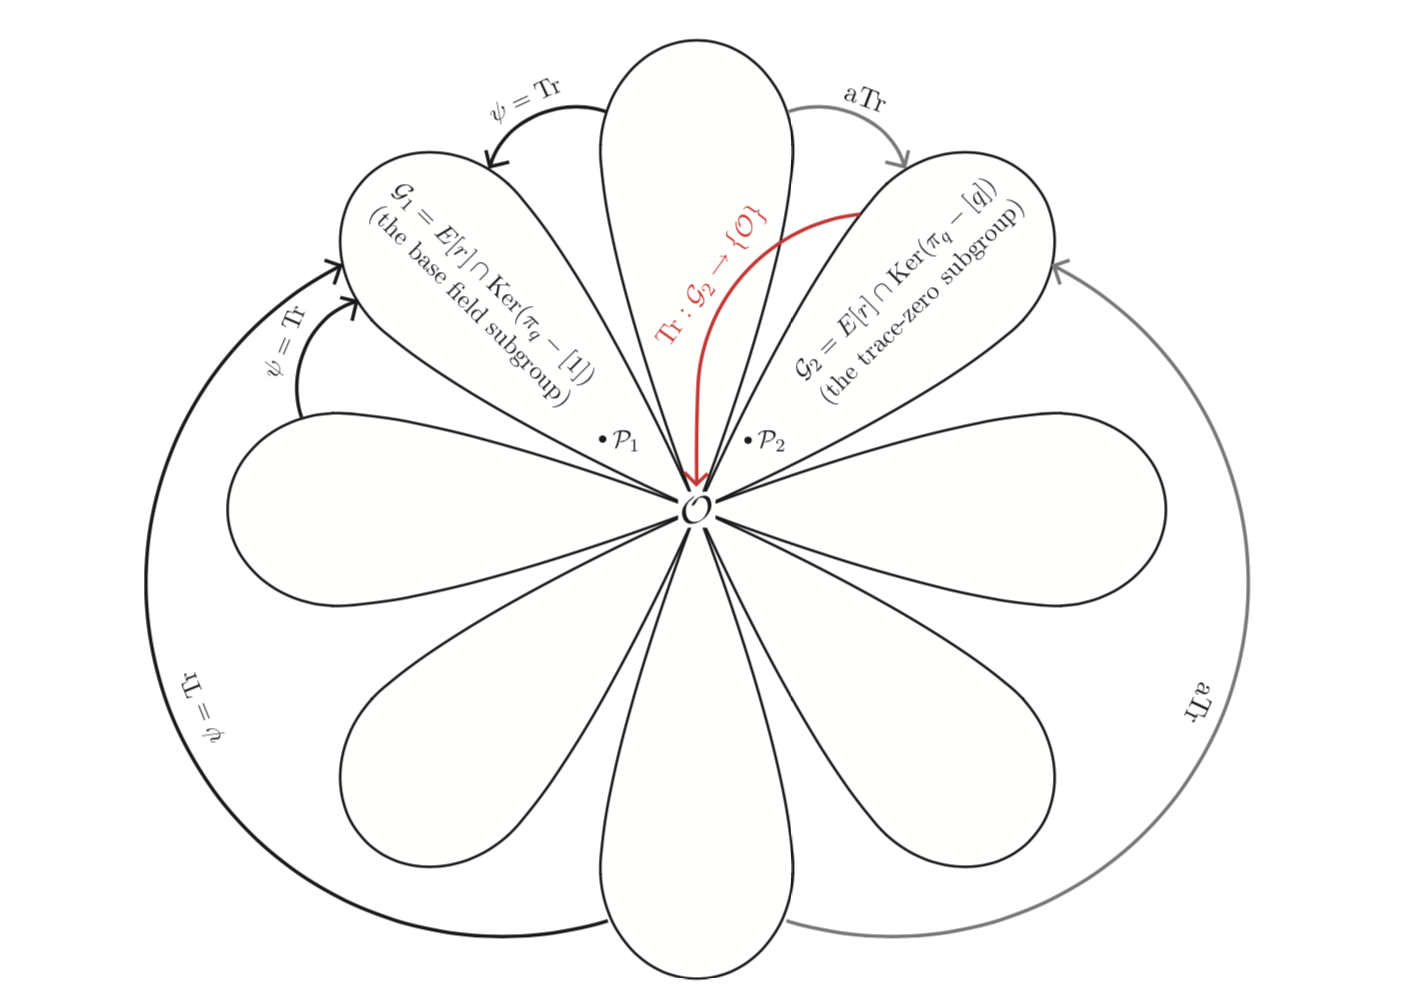
\includegraphics[width=0.8\textwidth]{../common/torsion.png}
	%\includegraphics[width=0.6\textwidth]{2.png}
	\caption{Torsion子群间的映射}
\end{figure}
对于supersingular的\ec,往往还存在一个映射能将$E(F_p)$中的点映射到$E(\fpk)$,称作distortion map。用它我们可以将$\mathcal{G}_1$的点映射到它之外。但实际中我们一般不做该选择,故此处不过多介绍。

对于具体的定义域选择存在著名的4种类型,这里我们介绍参考资料[2]中采用的第三种类型:选取$\mathbb{G}_1 = \mathcal{G}_1, \mathbb{G}_2 = \mathcal{G}_2$。则子群$E[r]$都能映射到pairing定义域中。\footnote{[2]中提到此时存在$\mathbb{G}_1$和$\mathbb{G}_2$的同构映射,且这个映射我们难以找出(但对手可能找出)。这可能会造成安全性问题。}

$\mathbb{G}_2$中的点可能存在难以表示的问题。Twisted curves提供了映射并表示$\mathbb{G}_2$中的点的方法。具体见参考资料[2]。
\subsection{Miller’s algorithm}
基于上述准备工作,我们可以介绍pairing函数的具体实现。

在此之前我们需要定义一个特别的函数,给定一个点$P\in E[r]$,定义函数$f_{r,p}$,其Divisor为
$$[f_{r,p}] = r[P]-r[\oo]$$
构造pairing函数的关键为找出一个实际可计算的满足上述条件的$f_{r,P}$。

具体计算方法为,定义一个函数族(一系列函数)$f_{m,P}, m \in \mathbb{Z}$,其Divisor为
$$f_{m,P} = m[P]-[mP]-(m-1)[\oo]	$$
注意到$m=r$时,因为$rP = \oo$,上述Divisor和$r[P]-r[\oo]$一致。

之后,我们可以通过递推关系
$$ f_{m+1,P} = f_{m,P}\cdot \frac{\ell_{mP,P}}{v_{(m+1)P}}$$
以及初始值$f_{0,P}=1$来计算。其中$\ell_{mP,P}$为经过$mP,P$两点的直线对应的函数,$v_{(m+1)P}$为经过点$(m+1)P$与$x$轴垂直的直线。

简要证明:注意到$[f_{m+1,P}]-[f_{m,P}] = [P]+[mP]-[(m+1)P]-[\oo]$,而$[\ell_{mP,P}] = [P]+[mP]+[-(m+1)P]-3[\oo]$,$[v_{(m+1)P}] = [(m+1)P]+[-(m+1)P]-2[\oo]$,后两者做差即得结论。

但是根据$m$从零开始递推时间复杂度过高。Miller's Algorithm给出了一种加速的算法:注意到
$$[f^2_{m,P}] =2m[P]-2[mP]-2(m-1)[\oo]$$
$$[f_{2m,P}] = 2m[P]-[2mP]-(2m-1)[\oo] $$
两者的差值为$2[mP]-[2mP]-[\oo]$,这个值同样可以由两条直线函数做商来得到,即
$$f_{2m,P} = f^2_{m,P}\cdot \frac{\ell_{mP,mP}}{v_{2mP}},$$
其中$\ell_{mP,mP}$为点$mP$在$E$上的切线对应的函数,$v_{2mP}$为经过点$(m+1)P$与$x$轴垂直的直线对应的函数。

该公式让我们能够通过$f_{m,P}$直接跳到$f_{m,2P}$,故最终计算$f_{r,P}$时能用类似二分求幂的方法来计算。具体见后面的算法介绍。
\subsection{Weil and Tate pairings}
最为著名的两个pairing函数为Weil和Tate。两者本质上类似,Tate在实际中更具有可用性,但这里我们先介绍Weil。

\textbf{给定$P,Q \in E(\fpk)[r]$,然后假设有Divisor $D_P, D_Q \in Div^0$满足$D_P \sim [P]-[\oo], D_Q \sim [Q]-[\oo]$且$D_P, D_Q$的support不相交(recall Weil reciprocity的限定条件),那么一定存在函数$f,g$,满足$[f] = rD_p$且$[g]=rD_Q$。}

\textbf{ Weil pairing $\omega_r: E(\fpk)[r] \times E(\fpk)[r] \rightarrow \mu_r$定义为
$$ w_r(P,Q) = \frac{f(D_Q)}{g(D_P)}$$
其中$\mu_r$为某个$r$次单位根($\mu_r^r =1$,定义在$\fpk$上)。
}

注:在实际展开计算$\omega_r$,我们仍需要选取$P,Q$分别来自上一章提到的$\mathcal{G}_1,\mathcal{G}_2$。但由于存在$E(\fpk)[r] \rightarrow \mathcal{G}_1,\mathcal{G}_2$且维持群运算的映射,我们可以认为定义域为$E(\fpk)[r]$。 对之后介绍的Tate pairing同理。

我们接下来简要介绍如何选取定义中用到的变量
\begin{itemize}
    \item 先根据Miller算法算出$f_{r,P},f_{r,Q}$ ($[f_{r,P}]=r[P]-r[O], [f_{r,Q}]=r[Q]-r[O]$)。
    \item 然后随机选取两个点$R,S \in E(\fpk)$,置$D_P = [P+R]-[R], D_Q = [Q+S]-[S]$。(注意到$[P]-[\oo]-D_P$能写成$[\frac{\ell_{P,R}}{v_{P+R}}]$,见下一节)
    \item 置$f = f_{r,P}/(\ell_{P,R}/v_{P+R})^3, g = f_{r,Q}/(\ell_{Q,S}/v_{Q+S})^3$,其中$\ell_{P,R}$为过$P,R$两点的直线对应的函数,$v_{P+R}$为经过点$P+R$与$x$轴垂直的直线对应的函数。对$\ell_{Q,S},v_{Q+S}$同理。
\end{itemize}
Tate pairing的不同之处在于,它要求某个输入点,如$Q$,来源于quotient group $E[\fpk]/rE(\fpk)$。但同时可以证明,只要$r^2 \| \#E(\fpk)$,$E[\fpk]/rE(\fpk)$可以被$E(\fpk)[r]$代表。故可以回归到和Weil pairing定义域相同的情形。

Tate pairing的具体定义如下:
\textbf{给定$P\in E(\fpk)[r]$,则存在函数$f$满足其Divisor为$[f]=r[P]-r[\oo]$。给定$Q \in E[\fpk]$为quotient group $E[\fpk]/rE(\fpk)$的一个代表点(事实上,可以忽略后半句)。假设有Divisor $D_Q \in Div^0$满足$D_Q \sim [Q]-[\oo]$,且support和$[f]$不相交。}

\textbf{Tate pairing $t_r: E(\fpk)[r]\times E(\fpk)/rE(\fpk) \rightarrow \fpk^*/(\fpk^*)^r$定义为
	$$ t_r(P,Q)= f(D_Q)$$
}
根据之前的定义,我们可以选择$f=f_{r,P}$,然后随机选取\ec 点$R$,置$D_Q=[Q+R]-[R]$,满足Tate pairing定义中的条件。

同时注意到,根据上述算法的得到的结果$t_r$可能看起来不相等(如计算$t_r(2P,Q)$和$t_r(P,2Q)$),但在$\fpk^*/(\fpk^*)^r$的定义域下是相等的(即两者的商是$r$次剩余类)。然而判断在$\fpk^*/(\fpk^*)^r$的定义域下是否相等也是一件很麻烦的事。解决的思路可以基于如下性质:如果两个数在$\fpk^*/(\fpk^*)^r$的定义域下相等,则它们的$\# \fpk/r=(q^k-1)/r$次方相等,且为$\fpk$下的$r$次单位根($\mu_r$)。故我们有下面的reduced Tate pairing,定义为(其他变量及条件与Tate pairing相同)
$$T_r(P,Q) = t_r(P,Q)^{\# \fpk/r} = f_{r,P}(D_Q)^{(q^k-1)/r}$$
我们总结完整的Miller's algorithm如下, 用于计算Tate pairing:

\begin{algorithm}[H]
	\caption{Miller's algorithm}%算法名字
	\KwIn{$P \in E(\fpk)[r]$, $D_Q = [2Q]-[Q]$($\sim [Q]-[O]$), $r=(r_{n-1}\cdots r_1r_0)_2$且$r_{n-1}=1$}
	\KwOut {$f_{r,P}(D_Q) \leftarrow f$ }
	\hrule
    $R \leftarrow P, f \leftarrow 1$.\;
    \For {$i=n-2$ down to $0$}
        { 计算直线$\ell_{R,R},v_{2R}$的函数\;
         $R \leftarrow 2R$\;
         $f \leftarrow f^2\cdot \frac{\ell_{R,R}}{v_{2R}}(D_Q)$\;
         \If {$r_i=1$}
         {
         	  计算直线$\ell_{R,P},v_{R+P}$的函数\;
         	  $R \leftarrow R+P$\;
         	  $f \leftarrow f\cdot \frac{\ell_{R,P}}{v_{R+P}}(D_Q)$\;
         }
   }
   \KwRet $f$.\;
	\label{alg:miller}
\end{algorithm}
上述算法有两个很重要的加速方法
\begin{itemize}
	\item 根据[BKLS02, Th. 1],只要$P,Q$线性无关,$k>1$,有
	$$ f_{r,P} (D_Q)^{(p^k−1)/r} = f_{r,P}(Q)^{(p^k−1)}/r$$
	这意味着计算关键的函数值时,直接在$Q$计算即可,省去了计算复杂的函数$D_Q$的麻烦。
	\item 另外一个优化方法叫denominator elimination,源于[BKLS02, Lemma 1]。他指出,我们在计算函数$\ell/v$时,可以直接把分母$v$去掉!这不仅大大减少了计算量,也省去了计算逆运算的麻烦。
\end{itemize}
根据上述方案,优化后的(BKLS-GHS版本)Miller算法描述如下:

\begin{algorithm}[H]
	\caption{The BKLS-GHS version of Miller’s algorithm for the Tate pair-
		ing.}
	\KwIn{$P \in \mathbb{G}_1$, $Q \in \mathbb{G}_2$, $r=(r_{n-1}\cdots r_1r_0)_2$且$r_{n-1}=1$}
	\KwOut{$f_{r,P}(Q)^{(p^k-1)/r}\leftarrow f$}
	\hrule
	$R \leftarrow P, f \leftarrow 1$.\;
	\For {$i=n-2$ down to $0$}
	{ 计算直线$\ell_{R,R}$的函数\;
		$R \leftarrow 2R$\;
		$f \leftarrow f^2\cdot \ell_{R,R}(Q)$\;
		\If {$r_i=1$}
		{
			计算直线$\ell_{R,P}$的函数\;
			$R \leftarrow R+P$\;
			$f \leftarrow f\cdot \ell_{R,P}(Q)$
		}
	}
	\KwRet $f \leftarrow f^{(q^k-1)/r}$.
	\label{alg:BKLS}
\end{algorithm}
参考资料[2]中还介绍了其他的优化方法,包括
\begin{itemize}
	\item 选择更为合适的映射空间(做点倍数运算$2P$更快)。
	\item 选择更为合适的扩展域(如$k=12$时,先做$2$次扩展,在做3次扩展,最后再做2次扩展)。
	\item 选择更为先进的ate pairing
	\item 选择低Hamming值的循环($r$)。
	\item 选择合适的方法计算最后的$(p^k-1)/r$次方
\end{itemize}
\subsection{选取pairing friendly的曲线}
之前提到,为了达到AES-128的安全级别,既要保证\ec 群$\mathbb{G}_1,\mathbb{G}_2$的规模在256位的级别,同时要保证目标群$\mathbb{G}_T$的规模在3248位的级别。简单的增加$k$仅能增加了后一部分的安全级别,但是大大提高了计算pairing的复杂度。

我们希望一个好的pairing能满足上述安全级别的同时使得参数尽可能小。其中一个衡量指标为$\rho-$value,定义为
$$ \rho = \frac{\log p}{\log r}$$
我们希望$\rho$尽可能接近1,即选取的子群$E[r]$的规模和质数$p$的规模一致。

有一系列曲线满足$\rho=1$,称作\textbf{BN curve}。该类曲线的$k$统一为12,很好的满足了安全性需求。

[FST10]进一步给出了期望满足的指标:
\begin{itemize}
	\item 存在质数$r \geq \sqrt{p}$且$r| \# E(\fp)$,(即$\rho \leq 2$),以及
	\item $k \leq \log_2(r)/8$
\end{itemize}
supersingular曲线通常比较容易满足上述条件,且$k \leq 6$,但是会牺牲计算pairing的效率。

还有一系列被称作\textbf{MNT curve}(非supersingular)也能很好的满足上述需求。事实上,MNT curve给出了构造一系列满足条件的曲线的方式。

值得一提的是,随机选择一个曲线大概率是不能够支持pairing的,故我们再用\ec 加密的时候不需要特意避免pairing的存在。相反,只有采用特定的方法小心选取才能找出pairing friendly的曲线。

至此,所有关于pairing的知识介绍完毕。
\newpage
\begin{appendices}
%\input{changelog.tex}
\end{appendices}

\end{document}
